\chapter{Specifikáció}

Az alábbi fejezet az alkalmazás alapvető működéséhez szükséges funkciókkal foglalkozik. Ezeknek korai lefektetése
és tisztázása fontos, hogy az implementáció során ne essünk overengineering\cite{Overengineering} vagy a hibásan implementált funkcionalitás csapdájába.

\section{Felhasználókezelés}

Az alkalmazásra legyen lehetőség regisztrálni, illetve a regisztrált felhasználóknak bejelentkezni, valamint a már bejelentkezett felhasználóknak kijelentkezni.
A regisztráció során a név, email cím és jelszó megadása kötelező, egy email címmel csak egy fiók hozható létre.
Bejelentkezni a név és email cím megadásával lehet.

\section{Könyvek listázása}

A rendszer biztosítja az elérhető könyvek listázását, a könyvek közötti kulcsszavas keresést, valamint
egy kiválasztott könyv részletes nézetét.

\section{Kosár}

A könyveket a webshopokban megszokott módon kosárba helyezhetünk (egy könyvből akár többet, de maximum az elérhető mennyiségnek megfelelőt).
A kosár tartalmát lehetőségünk van listázni, a benne lévő elemeket szerkeszteni (darabszámot növelni és csökkenteni, könyvet eltávolítani, vagy a teljes kosarat kiüríteni).

\section{Kölcsönzés kezelése}

A kosárba helyezett könyveket le tudjuk adni a visszavitel időpontjának megadásával, ekkor a kölcsönzés ``Függőben'' állapotba kerül.

Ezután a kölcsönzés oldalán az alkalmazás adminisztrátoraival lehetőség van átvételi időpont egyeztetésére a kölcsönzéshez fűzhető kommenteken keresztül.
A kölcsönzést illetve a hozzá tartozó kommenteket csak az kölcsönző, illetve megfelelő jogosultsággal rendelkező adminisztrátor láthatja

\section{Admin funkcionalitás}

Az alkalmazás adminjainak lehetősége van könyvek illetve kategóriák hozzáadására, szerkesztésére és törlésére.

Ezen kívül frissíthetik a kölcsönzés állapotát, törölhetik azt, valamint hozzászólást fűzhetnek a kölcsönzésekhez.


\section{Use-case diagram}

A fenti követelményeket az alábbi use-case diagramban foglaltam össze. Ebben megkülönböztetek nem bejelentkezett illetve bejelentkezett felhasználót (utóbbi mindenképp rendelkezik egy szerepkörrel).

\begin{figure}[!ht]
  \centering
  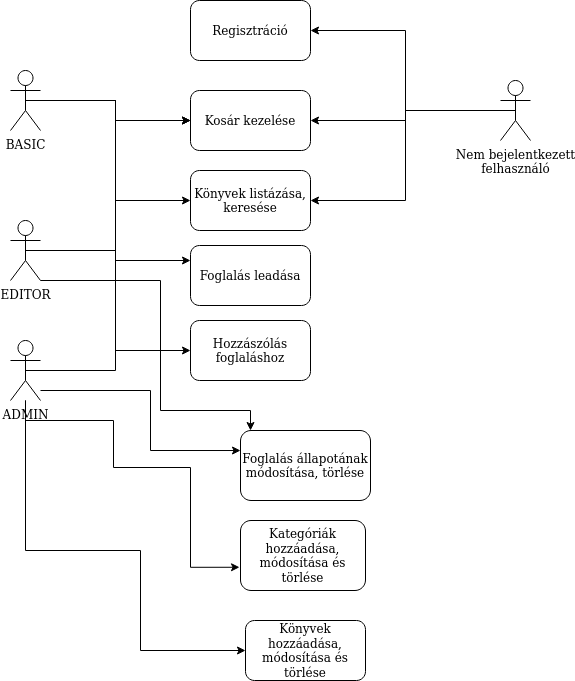
\includegraphics[width=100mm, keepaspectratio]{figures/usecase.png}
  \caption{Az alkalmazáshoz tartozó use-case diagram}
  \label{fig:UseCase}
\end{figure}
